\documentclass{standalone}
\usepackage{tikz}
\usepackage{ctex,siunitx}
\setCJKmainfont{Noto Serif CJK SC}
\usepackage{tkz-euclide}
\usepackage{amsmath}
\usetikzlibrary{patterns, calc}
\usetikzlibrary {decorations.pathmorphing, decorations.pathreplacing, decorations.shapes,}
\begin{document}
\small
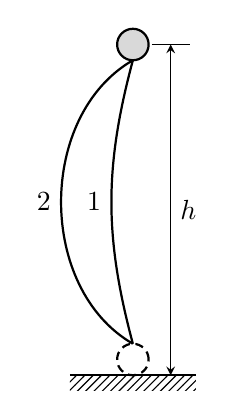
\begin{tikzpicture}[>=stealth,thick,scale=0.8]
  \fill [pattern = north east lines] (0,-.25) rectangle (2,0);
  \draw (0,0)--(2,0);
  \draw [densely dashed] (1,.25) circle (.25);
  \draw [fill=gray!30] (1,5.25) circle (.25);
  \draw [thin](1.3,5.25)--(1.9,5.25);
  \draw [thin,<->](1.6,5.25)--(1.6,0)node [midway,right]{$h$};
  \draw (1,5) [bend right=60] to node [left]{2} (1,.5);
  \draw (1,5) [bend right=15] to node [left]{1} (1,.5);
\end{tikzpicture}
\end{document}